% ----------------------------------------------------------

\section{\textbf{Referencial Bibliográfico}}%\label{cap:desenvolvimento}
% ----------------------------------------------------------
%Deve-se inserir texto entre as seções.
%--------Adicionar uma descrição melhor para a parte de referencias---------------

Dentre as principais bibliotecas disponíveis pela ferramenta Python, foram utilizadas durante o código as seguintes bibliotecas Pandas, Numpy, PYMuPDF e FDPF. Pandas teve sua utilização na estruturação dos dados utilizados em modelo Data Frame, Numpy foi utilizado para formatação de tipos de dados estruturados, PYMuPDF foi utilizado para a leitura das notas que virão em PDF, FPDF foi utilizado para formalizar e formatar o resultado final para melhor visualização do usuário em um arquivo PDF. Todas essas bibliotecas foram pré instaladas via \textit{Requiriments}, dando uma maior facilidade de utilização do código ao usuário.


\subsection{Python}\label{sec:Python}
%    \ABNTEXfontereduzida
%
Como é dito por \textcite{borges2014python} a linguagem Python inclui estruturas de alto nível e uma grande e vasta coleção de bibliografia e além disso a grande abrangência de \textit{frameworks} que podem ser utilizados em quaisquer projetos. Também é citado pelo autor que sua linguagem sendo ela uma das mais atuais no mercado, veio derivada de várias outras e assim pode ter entradas de códigos de outras fontes, como por exemplo C, C++ e JavaScript se tornando assim uma ferramenta versátil de simples manuseio do usuário que não tem conhecimento em programação ou até mesmo sobre a própria linguagem.

\par Por ser uma linguagem de código aberto ela possui vasta documentação em grandes comunidades da internet, segundo dados do \textcite{StackOverflow}
podemos ver na \autoref{fig:Fig_1} que Python é a linguagem que mais possui perguntas no fórum e possui um crescimento acentuado nas perguntas atuais.

\begin{figure}[h]
    \caption{\label{fig:Fig_1}Linguagens com maior fluência de pesquisas.}
    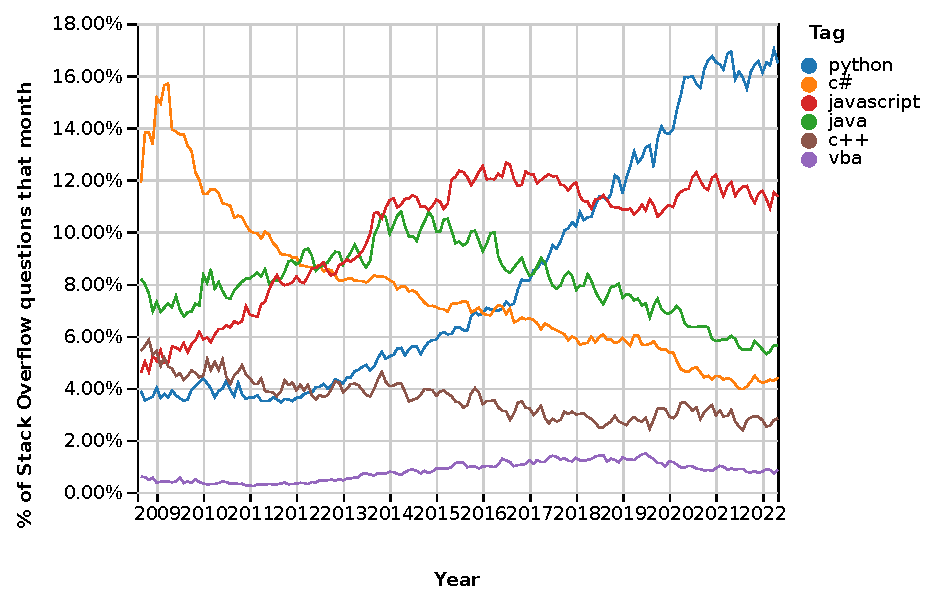
\includegraphics[width=\textwidth]{TCC_Renda/figuras/Graph1.eps}
    \fonte{\cite{StackOverflow}2009-2022}
\end{figure}

\subsection{Pandas}\label{sec:Pandas}

\par Segundo \textcite{mckinney2019} ao utilizar a ferramenta Pandas é oferecido várias estruturas para dados de alto nível e funções, o mais importante é ele ser um dado estruturado ou tabulado de forma fácil e expressiva.
%---------------------REVER---------------------------------
\par Pandas teve seu início de funcionamento a partir do ano de 2010, pandas vem ajudando projetistas e programadores de Python fazendo que seja um ambiente mais eficaz para a análise de dados.
\par O modelo que iremos utilizar nesse trabalho/projeto será o DataFrame, utilizado para estruturar dados e tabular, orientação de colunas, com rótulos (\textit\textbf{lábels}) tanto para linhas quanto para colunas e também foi utilizado Series, como um objeto array unidimensional (exemplo seria um rótulo).
%---------------------REVER---------------------------------
\par A combinação das ideias de alto processamento de \textit{arrays} utilizado no Numpy é utilizado no Pandas só que de forma mais flexíveis para ser fácil a manipulação dos dados nas planilhas de bancos de dados relacionados, um exemplo seria o SQL.
\par Pandas também disponibiliza muitas funcionalidades sofisticadas de formatação, manipulação de dados, agregações e seleções de subconjuntos de dados. Como por exemplo a manipulação de dados na analise de dados e sua limpeza e preparação para a utilização final em contas e afins.
\par Algumas funcionalidades citadas por \textsc{\cite[p.12]{mckinney2019}} seriam:

\begin{citacao}
        \par - Estruturas de dados com eixos nomeados, com suporte para alinhamento automático ou explícito de dados – isso evita erros comuns resultantes de dados desalinhados e possibilita trabalhar com dados indexados de modo diferente, provenientes de origens distintas;
        \par - Funcionalidade para séries temporais integradas;
        Mesmas estruturas de dados para lidar com séries de dados tanto temporais quanto não temporais;
        \par - Operações aritméticas e reduções que preservem metadados;
        \par - Tratamento flexível para dados ausentes;
        \par - Combinações (\textit{merge}) e outras operações relacionais que se encontram em bancos de dados populares (baseados em SQL, por exemplo).
\end{citacao}

\subsection{Numpy}\label{sec:Numpy}
A biblioteca Numpy como é dito por \textcite{mckinney2019}, é uma ferramenta que oferece o código aglutinador utilizado para estruturas de dados, como por exemplo para algorítimos e é utilizado para várias aplicações com uso de números(dados numéricos).
\par Dentro da própria ferramenta podemos encontrar os recursos:

\begin{itemize}
    \item Utilização de Arrays multidimensional chamando \textit{ndarray} para ser mais rápido e de maior eficiência;
    \item Contém funcionalidade de multiprocessamento de informação de dados em várias arrays ao mesmo tempo e/ou em uma única;
    \item Contém a ferramenta de leitura e gravura de conjuntos de dados de acordo com a array no disco;
    \item operações de álgebra linear, transformadas de Fourier e geração de números aleatórios;
    \item Utiliza uma API C já treinada tendo sua permissão de utilização de outras linguagem no mesmo código como por exemplo C ou C++, para que tenham permissões de acesso nas estruturas de dados e outros processamentos de dados feito pelo \textit{Numpy}
\end{itemize}
%---------------------REVER---------------------------------
\par De forma não exclusiva os processamentos ágeis de \textit{arrays} dentro do próprio NumPy para acrescentar ao \textit{Python}, como citado nas funcionalidades, ele tem sua maior disponibilidade em análise de dados em forma de contêiner, sendo assim possível que todo dado analisado por ele no código possa ser passado para outro programa,algoritmo, em forma de biblioteca. Focando em dados numéricos, as arrays do \textit{Numpy} tem sua maior eficiência em armazenamento e manipulação de dados em comparação a outras ferramentas que funcionam em forma de \textit{built-in} (embutidas) pelo Python.
Por conta dessa funcionalidade, os dados que vierem de dados de baixo nível, como C e Fortran, podem ser utilizados e operar em uma \textit{array} do \textit{NumPy} sem que ela seja copiado os dados de outra representação da memória.
%---------------------REVER---------------------------------

\par Fazendo assim que as funcionalidades do próprio numpy em forma de processamento numérico não são acusadas pelo \textit{Python}e assim as estruturas do \textit{Numpy} podem ser utilizados como principais ou tem sua meta uma de comunicar com outros sistema de uma forma mais suave com a utilização do \textit{NumPy}.






\subsection{PyMuPDF}\label{sec:Fitz}

\par Ao se utilizar a ferramenta-modulo Fitz proveniente da biblioteca por por PyMuPDF e disponibilizado por \textcite{MUPDF}, é possível que possa puxar valores de planilhas do Excel e assim podendo ser colocados em seu código de forma estruturada e também podendo com isso utilizar em bases com grandes quantidades de dados.
\par Com a ferramenta PyMuPDF podem ser acessados também arquivos com as extensões ".pdf" “.xps”, “.oxps”, “.cbz”, “.fb2” or “.epub”.
\par Ferramenta disponível tanto para Mac quanto Windowns e Linux com Python.
\par Com seu fácil manuseio e de forma mais simples, utilizando scripts que podem ser configurados de outras linguagens como por exemplo C e C++, sendo assim editável as instancias que irá puxar da planilha em si.
\par Podendo extrair fotos, cores, links e compressões de página, e assim deixando o dado o mais "mastigado" possível para o funcionamento do código em geral.

\subsection{DataFrame}\label{sec:dataframe}

\par De acordo com \textcite{Petrou2017-no} todo dado em um disco de memória é tornado em um \textit{DataFrame} usando apenas uma variável que está disponível na linguagem Pandas,descrito em \autoref{sec:Pandas}, o comando em questão seria \textit{"pandas.DataFrame()"} sendo ela uma função. A saída de todas as colunas e o índex estariam em negrito deixando em um formato de melhor leitura para o usuário. Durante essa conversão os termos "\textit{Index Label}" e "\textit{Collumn Name}"  são referidos ao número individual dos membros do índice e da coluna em questão.
\begin{figure}[!]
    \caption{\label{fig:Fig_2}Estrutura de DataFrame.}
    \begin{center}
    \resizebox{\columnwidth}{!}{
    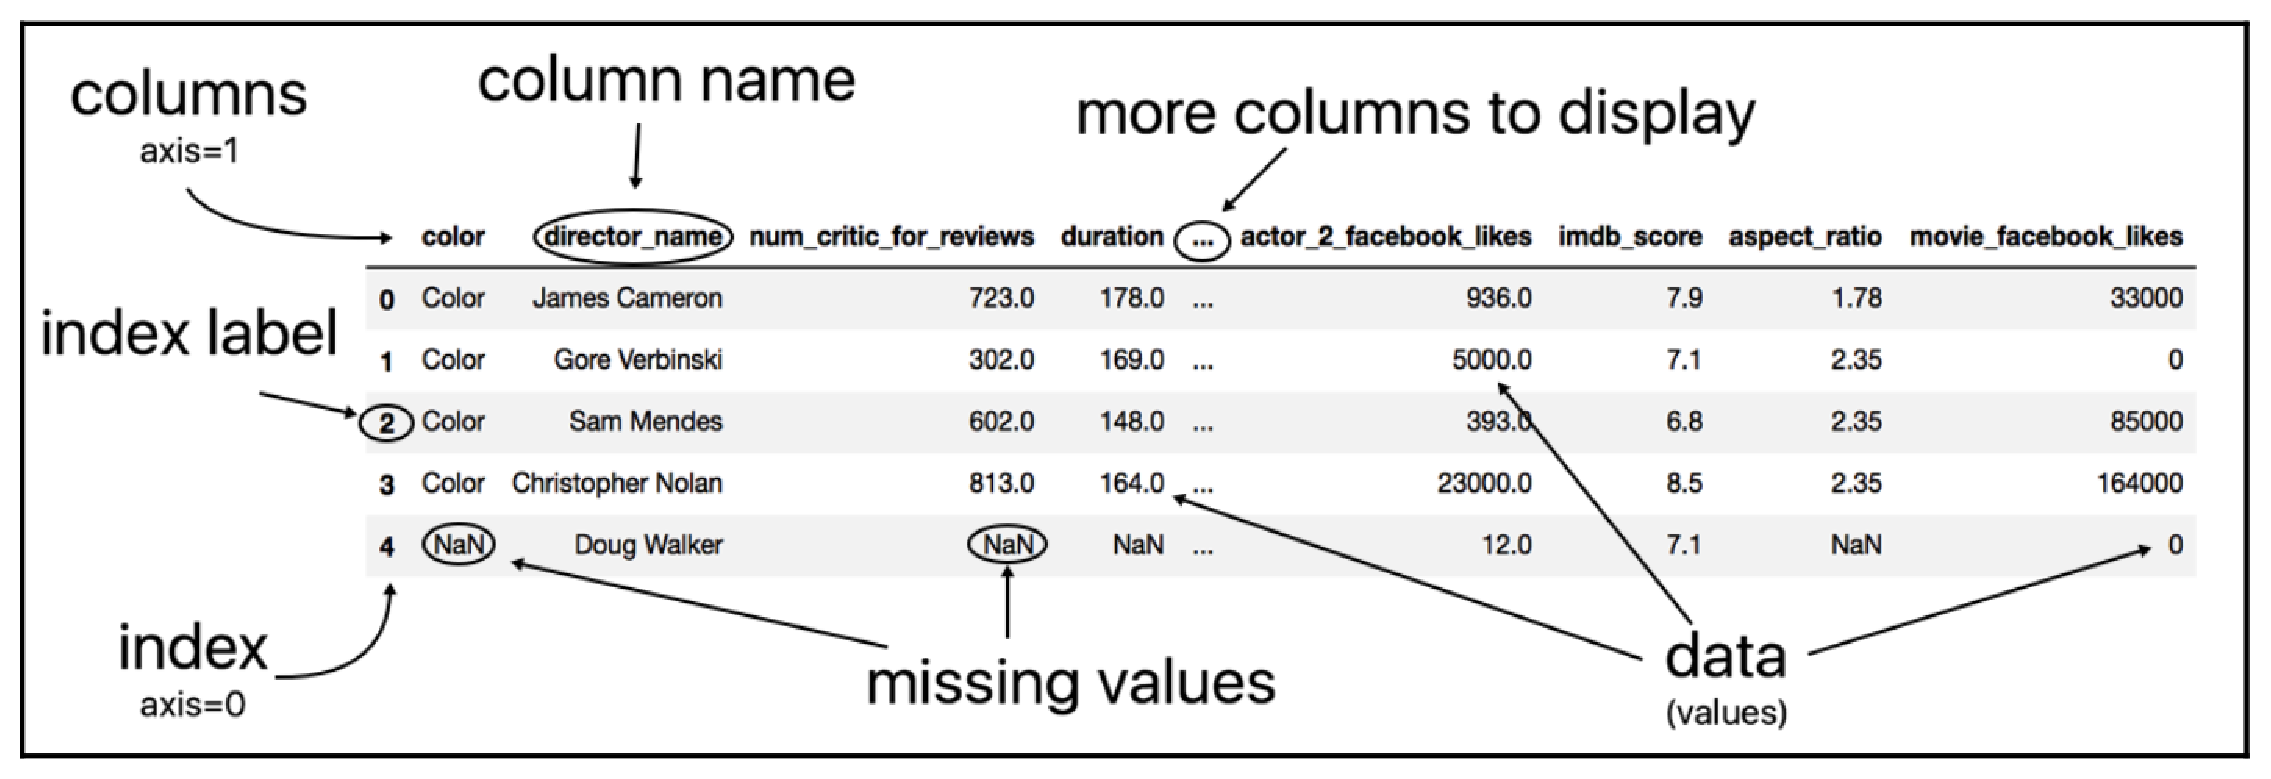
\includegraphics[width=\textwidth]{TCC_Renda/figuras/Dataframe.eps}
    }\end{center}
	\fonte{\cite[P.17]{Petrou2017-no}}
\end{figure}
\par O termo \textit{index} é referido à todos os rótulos de indicies como um todo, assim como o termo colunas se refere a todas as colunas
nomes como um todo.

\par A coluna do índice tem uma serventia em particular, e essa tem a função de prover rótulos para as colunas e as informações que entraram ao \textit{DataFrame}. Esses rótulos permitem que de forma direta e mais simples, possam ser acessados esses dados e sendo ele de diferentes locais em que o dado for colocado.

\par Quando vários tipos de \textit{DataFrames} são combinados esses indicies são alinhados primeiramente antes de qual quer tipo de cálculo seja feito. Disse \cite{Petrou2017-no} que,"Coletivamente, as colunas e o índice são conhecidos como os eixos."

\par Dado os Dados em que o \textit{DataFrame} sempre estão em forte regulares e também são componentes totalmente independentes tanto das colunas quanto do índice.
Já na ferramenta Pandas é utilizado o NaN(\textit{Not a Number}) para ser utilizado a representação dos valores que não são encontrados pela busca de dados.
\par Olhando para \autoref{fig:Fig_2} , podemos observar que a coluna de cores tem apenas valores de forma (\textit{"String"}), é utilizado o NaN para representar um valor ausente.

	\begin{figure}[ht]
    \caption{\label{fig:Fig_4}Fluxograma do trabalho.}
    \begin{center}
    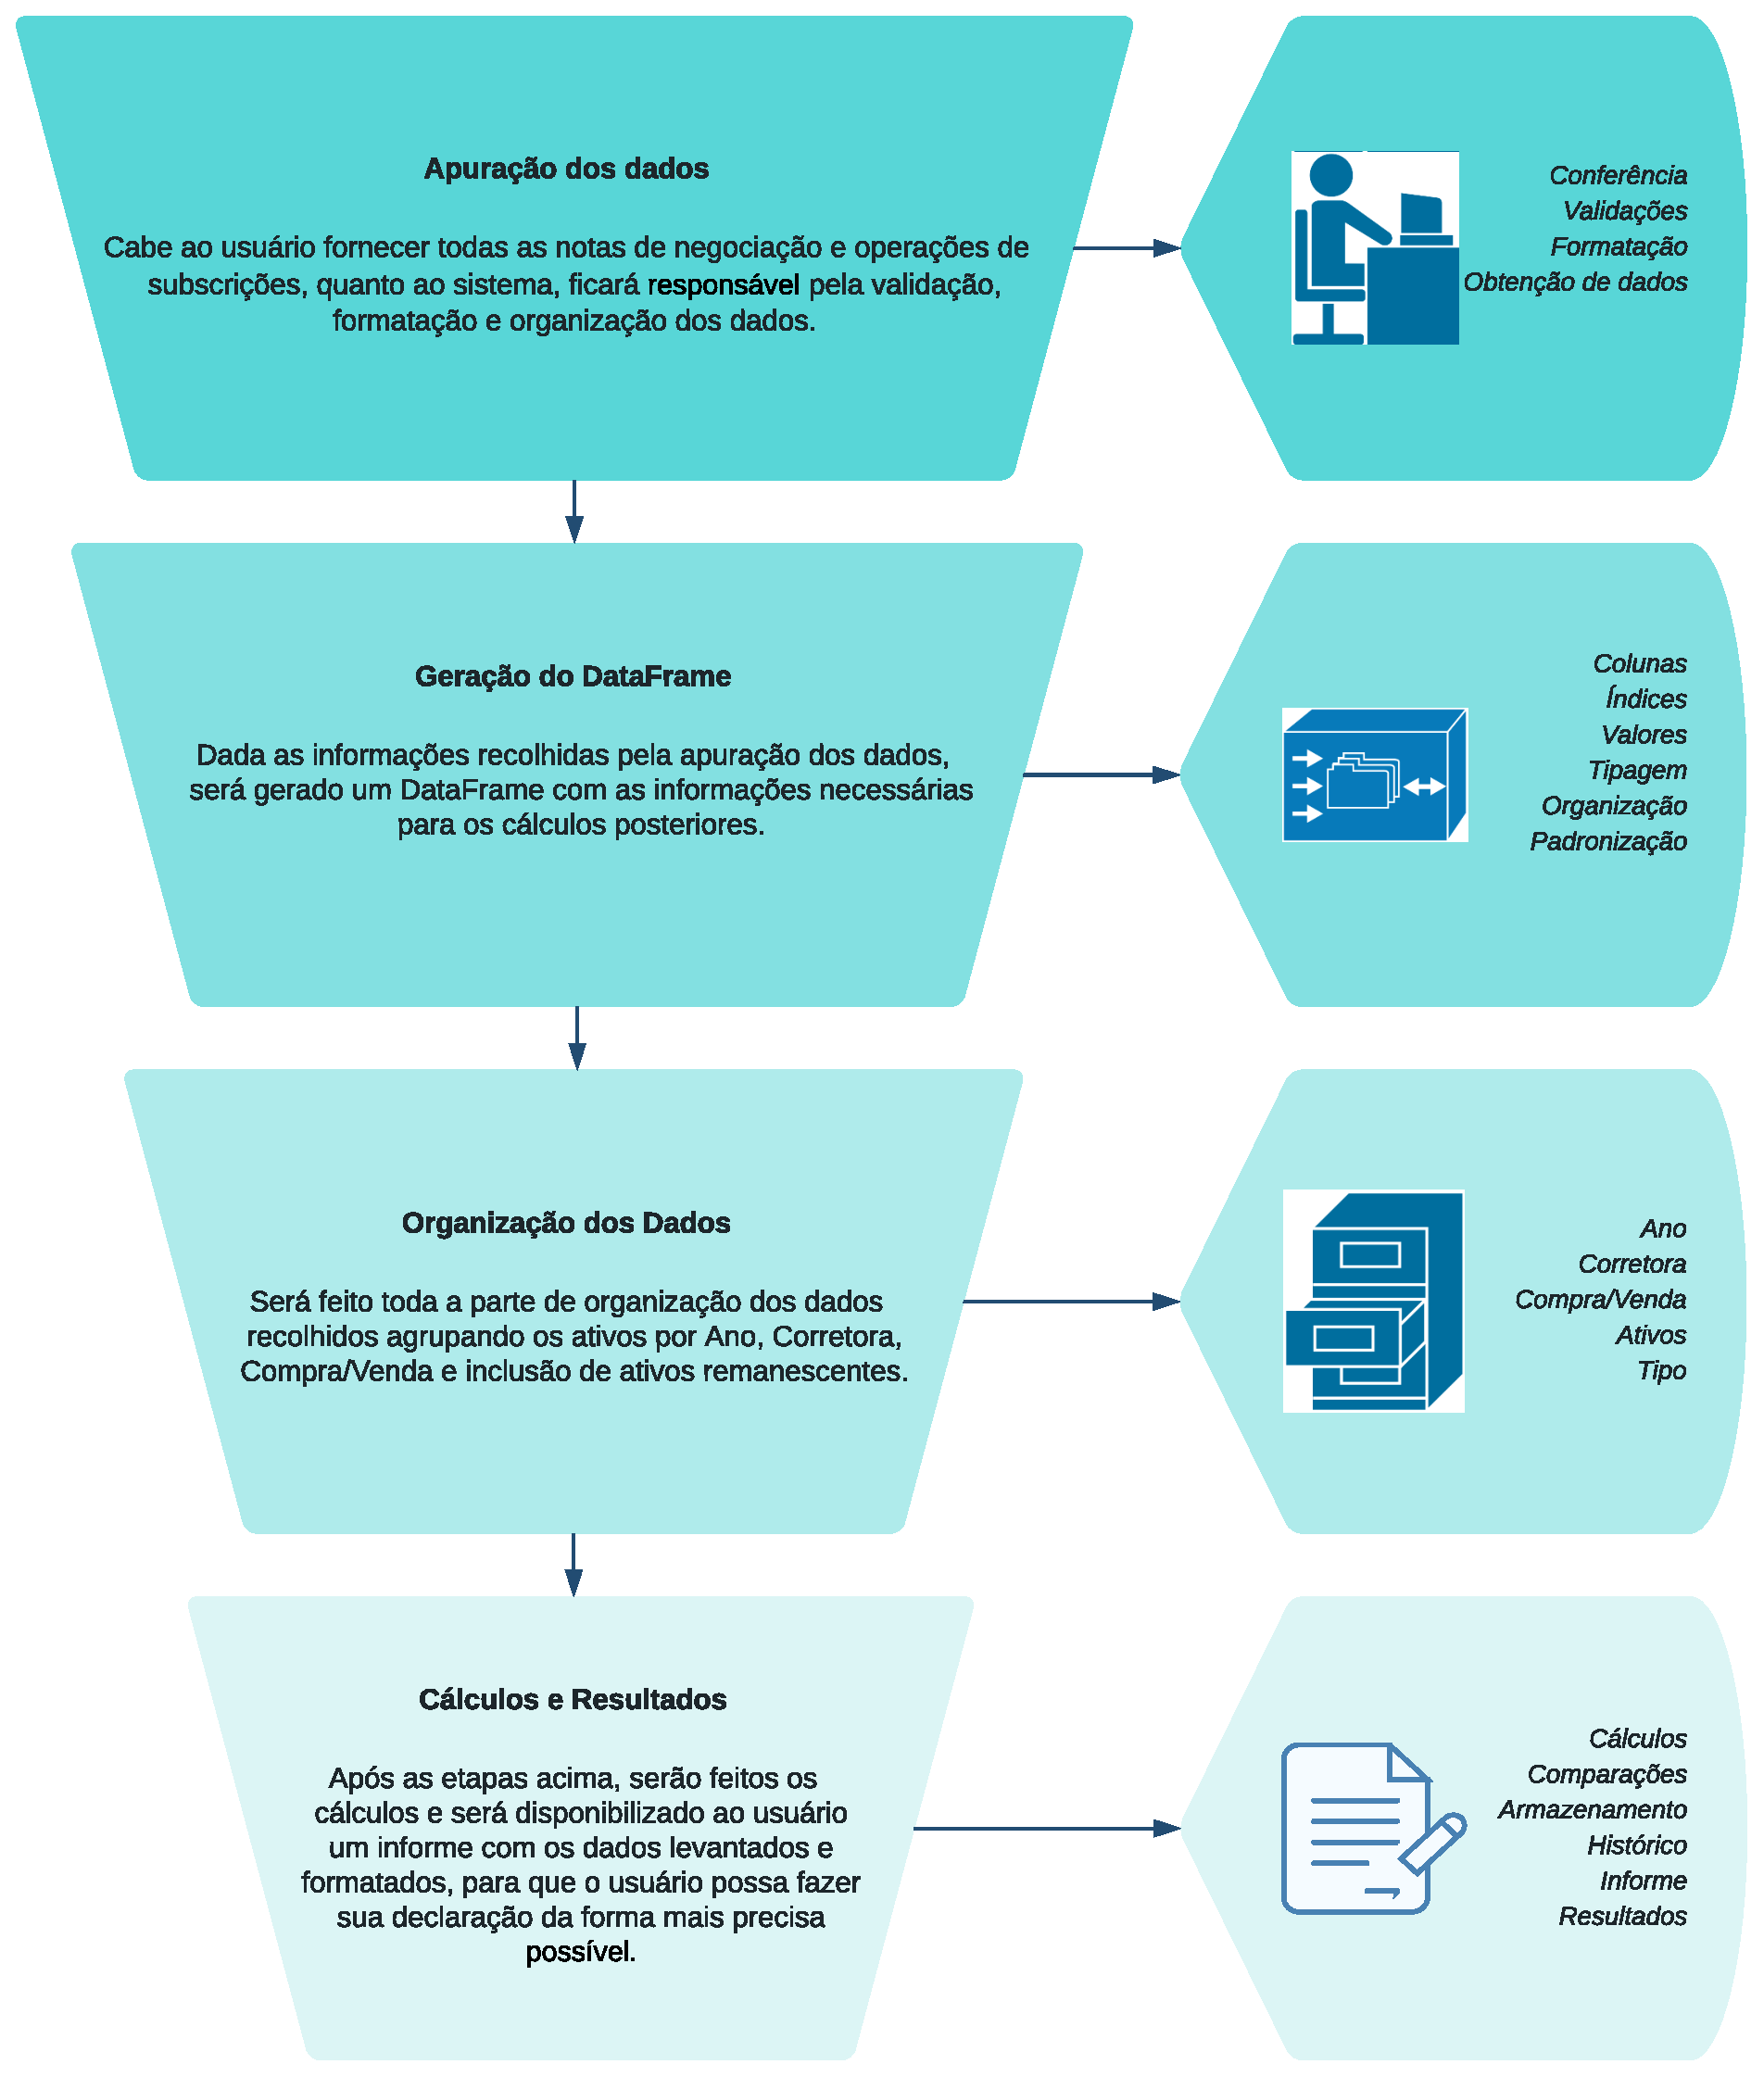
\includegraphics[scale=0.45]{TCC_Renda/figuras/TCC Fluxograma V5.eps}
    \end{center}
	\fonte{Autores do trabalho}
    \end{figure}